\documentclass[border={0.000000bp 0.000000bp 0.000000bp 0.000000bp}, 11pt]{standalone}
\pdfinfoomitdate=1
\pdftrailerid{}
\pdfsuppressptexinfo=1
\pdfinfo{ /Creator () /Producer () }

\usepackage{tikz}
\usepackage{xcolor}
\usetikzlibrary{shapes.misc}
\usetikzlibrary{backgrounds}

\definecolor{dotColorA}{HTML}{000000}
\definecolor{dotColorB}{HTML}{000000}
\definecolor{dotColorC}{HTML}{000000}
\definecolor{dotColorD}{HTML}{000000}
\definecolor{dotColorE}{HTML}{000000}

\definecolor{labelBgColorA}{HTML}{FFFFFF}
\definecolor{labelBgColorB}{HTML}{FFFFFF}
\definecolor{labelBgColorC}{HTML}{FFFFFF}
\definecolor{labelBgColorD}{HTML}{FFFFFF}
\definecolor{labelBgColorE}{HTML}{FFFFFF}

\definecolor{labelTextColorA}{HTML}{000000}
\definecolor{labelTextColorB}{HTML}{000000}
\definecolor{labelTextColorC}{HTML}{000000}
\definecolor{labelTextColorD}{HTML}{000000}
\definecolor{labelTextColorE}{HTML}{000000}

\definecolor{linkColorA}{HTML}{000000}
\definecolor{linkColorB}{HTML}{000000}
\definecolor{linkColorC}{HTML}{000000}
\definecolor{linkColorD}{HTML}{000000}
\definecolor{linkColorE}{HTML}{000000}

\def\textA{\textsc{bocpd}}
\def\textB{\textsc{bocpdms}}
\def\textC{\textsc{ecp}}
\def\textD{\textsc{kcpa}}
\def\textE{\textsc{zero}}

\begin{document}
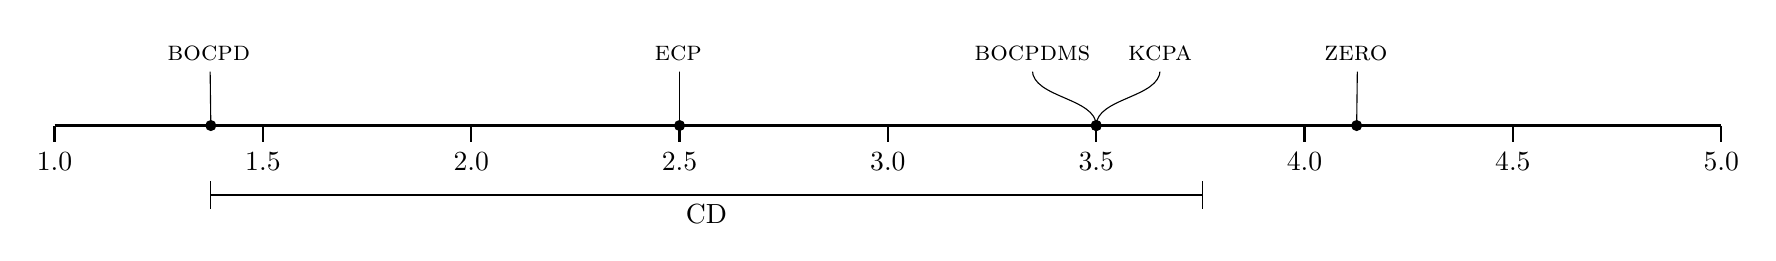
\begin{tikzpicture}[x=1bp,y=-1bp]

% shift for the margin
\begin{scope}[shift={(0, 0)}]
% main layer
\begin{scope}[shift={(0, 75)}]
% axis
\begin{scope}
\draw[very thick] (0, 0) -- (600, 0);
\end{scope}

% axis layer
\begin{scope}
\begin{scope}[shift={(0, 0)}]
\draw[thick] (0, 0) -- (0, -6pt)
node[anchor=north] {1.0};
\end{scope}
\begin{scope}[shift={(75, 0)}]
\draw[thick] (0, 0) -- (0, -6pt)
node[anchor=north] {1.5};
\end{scope}
\begin{scope}[shift={(150, 0)}]
\draw[thick] (0, 0) -- (0, -6pt)
node[anchor=north] {2.0};
\end{scope}
\begin{scope}[shift={(225, 0)}]
\draw[thick] (0, 0) -- (0, -6pt)
node[anchor=north] {2.5};
\end{scope}
\begin{scope}[shift={(300, 0)}]
\draw[thick] (0, 0) -- (0, -6pt)
node[anchor=north] {3.0};
\end{scope}
\begin{scope}[shift={(375, 0)}]
\draw[thick] (0, 0) -- (0, -6pt)
node[anchor=north] {3.5};
\end{scope}
\begin{scope}[shift={(450, 0)}]
\draw[thick] (0, 0) -- (0, -6pt)
node[anchor=north] {4.0};
\end{scope}
\begin{scope}[shift={(525, 0)}]
\draw[thick] (0, 0) -- (0, -6pt)
node[anchor=north] {4.5};
\end{scope}
\begin{scope}[shift={(600, 0)}]
\draw[thick] (0, 0) -- (0, -6pt)
node[anchor=north] {5.0};
\end{scope}
\end{scope}

% link layer
\begin{scope}
\draw[color=linkColorA, thin] (56.25, 0) .. controls
(56.25, -10.0) and (56.0, -10.0) .. (56.0, -20.0);
\draw[color=linkColorB, thin] (375.0, 0) .. controls
(375.0, -10.0) and (352.0, -10.0) .. (352.0, -20.0);
\draw[color=linkColorC, thin] (225.0, 0) .. controls
(225.0, -10.0) and (225.0, -10.0) .. (225.0, -20.0);
\draw[color=linkColorD, thin] (375.0, 0) .. controls
(375.0, -10.0) and (398.0, -10.0) .. (398.0, -20.0);
\draw[color=linkColorE, thin] (468.75, 0) .. controls
(468.75, -10.0) and (469.0, -10.0) .. (469.0, -20.0);
\end{scope}

% label layer
\begin{scope}
\begin{scope}[shift={(35, -34)}]
\fill[color=labelBgColorA, rounded corners=2pt]
(0, 0) rectangle (41, 14.62708) node[midway, yshift=-.75bp, anchor=center, text=labelTextColorA] {\strut \textA};
\end{scope}
\begin{scope}[shift={(325, -34)}]
\fill[color=labelBgColorB, rounded corners=2pt]
(0, 0) rectangle (54, 14.62708) node[midway, yshift=-.75bp, anchor=center, text=labelTextColorB] {\strut \textB};
\end{scope}
\begin{scope}[shift={(211, -34)}]
\fill[color=labelBgColorC, rounded corners=2pt]
(0, 0) rectangle (27, 14.62708) node[midway, yshift=-.75bp, anchor=center, text=labelTextColorC] {\strut \textC};
\end{scope}
\begin{scope}[shift={(381, -34)}]
\fill[color=labelBgColorD, rounded corners=2pt]
(0, 0) rectangle (34, 14.62708) node[midway, yshift=-.75bp, anchor=center, text=labelTextColorD] {\strut \textD};
\end{scope}
\begin{scope}[shift={(452, -34)}]
\fill[color=labelBgColorE, rounded corners=2pt]
(0, 0) rectangle (33, 14.62708) node[midway, yshift=-.75bp, anchor=center, text=labelTextColorE] {\strut \textE};
\end{scope}
\end{scope}

% dots
\begin{scope}
\draw node [circle, inner sep=0pt, minimum size=4bp, 
fill=dotColorA] at (56.250000, 0) {};
\draw node [circle, inner sep=0pt, minimum size=4bp, 
fill=dotColorB] at (375.000000, 0) {};
\draw node [circle, inner sep=0pt, minimum size=4bp, 
fill=dotColorC] at (225.000000, 0) {};
\draw node [circle, inner sep=0pt, minimum size=4bp, 
fill=dotColorD] at (375.000000, 0) {};
\draw node [circle, inner sep=0pt, minimum size=4bp, 
fill=dotColorE] at (468.750000, 0) {};
\end{scope}

% Critical difference
\def\posBest{56.2500000000000000}
\def\posCD{413.1340352124062747}
\begin{scope}
\draw (\posBest, 30) -- (\posBest, 20);
\draw (\posBest, 25) --node[below] {CD} (\posCD, 25);
\draw (\posCD, 30) -- (\posCD, 20);
\end{scope}

\end{scope}
\end{scope}
\end{tikzpicture}
\end{document}